
\begin{figure}
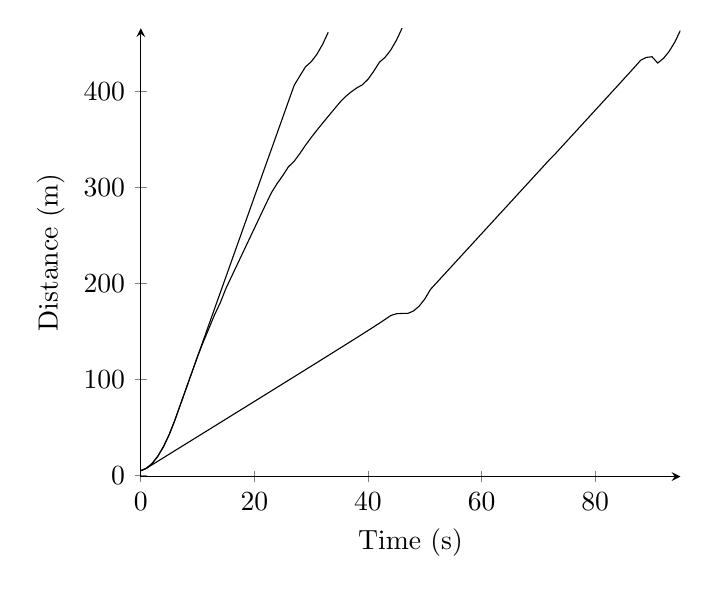
\begin{tikzpicture}
\begin{axis}[
legend style={anchor=west},
axis x line=bottom,
axis y line=left,
ymin=-1,
xlabel=Time (s),
ylabel=Distance (m),
]
\addplot[] coordinates {
(0, 5.1)
(1, 7.6)
(2, 12.6)
(3, 20.1)
(4, 30.1)
(5, 42.6)
(6, 57.6)
(7, 74.2)
(8, 90.8)
(9, 107.4)
(10, 124.0)
(11, 139.027223027)
(12, 153.173429236)
(13, 167.427306285)
(14, 179.907918049)
(15, 194.888529812)
(16, 207.373398485)
(17, 219.858305023)
(18, 232.343256108)
(19, 244.828260097)
(20, 257.313327572)
(21, 269.798472142)
(22, 282.283711602)
(23, 294.404236242)
(24, 303.897134344)
(25, 312.206247681)
(26, 321.417866532)
(27, 327.07915298)
(28, 335.100439427)
(29, 343.815241427)
(30, 351.825322903)
(31, 359.397666906)
(32, 366.714711048)
(33, 373.893519471)
(34, 381.009780535)
(35, 388.121532235)
(36, 394.222772429)
(37, 399.141110522)
(38, 403.391833589)
(39, 406.673074683)
(40, 412.454315777)
(41, 420.735556872)
(42, 430.100885294)
(43, 435.223356983)
(44, 442.845828672)
(45, 452.968300361)
(46, 465.590772049)
};
\addplot[] coordinates {
(0, 5.1)
(1, 7.6)
(2, 11.2586202875)
(3, 14.9174172996)
(4, 18.5764028533)
(5, 22.2355898444)
(6, 25.8949923737)
(7, 29.5546258913)
(8, 33.2145073619)
(9, 36.8746554558)
(10, 40.5350907689)
(11, 44.1958360777)
(12, 47.8569166366)
(13, 51.5183605248)
(14, 55.1801990534)
(15, 58.8424672449)
(16, 62.5052044018)
(17, 66.1684547817)
(18, 69.8322684065)
(19, 73.4967020346)
(20, 77.1618203378)
(21, 80.827697335)
(22, 84.49441815)
(23, 88.1620811833)
(24, 91.8308008162)
(25, 95.5007108075)
(26, 99.1719685992)
(27, 102.84476083)
(28, 106.519310474)
(29, 110.195886198)
(30, 113.874814786)
(31, 117.556497897)
(32, 121.241435018)
(33, 124.930255533)
(34, 128.618861715)
(35, 132.31310684)
(36, 136.014491813)
(37, 139.724908687)
(38, 143.447001063)
(39, 147.184591324)
(40, 150.943449426)
(41, 154.732788467)
(42, 158.568499082)
(43, 162.481310517)
(44, 166.543253205)
(45, 168.455330147)
(46, 168.752634192)
(47, 168.752634192)
(48, 171.252634192)
(49, 176.252634192)
(50, 183.752634192)
(51, 193.752634192)
(52, 200.194644587)
(53, 206.636664421)
(54, 213.07869449)
(55, 219.520735681)
(56, 225.962788988)
(57, 232.404855525)
(58, 238.846936549)
(59, 245.291246485)
(60, 251.735648877)
(61, 258.180153427)
(62, 264.624771244)
(63, 271.069515109)
(64, 277.514399802)
(65, 283.959442508)
(66, 290.404663329)
(67, 296.850085928)
(68, 303.295738356)
(69, 309.74165412)
(70, 316.187873575)
(71, 322.634445775)
(72, 329.081430942)
(73, 335.088903851)
(74, 341.536067768)
(75, 347.983619784)
(76, 354.43164577)
(77, 360.880258983)
(78, 367.329611952)
(79, 373.779915158)
(80, 380.231467518)
(81, 386.684708452)
(82, 393.140311806)
(83, 399.59936725)
(84, 406.063762486)
(85, 412.537088042)
(86, 419.024794644)
(87, 425.551381812)
(88, 432.206889574)
(89, 435.202295352)
(90, 435.908445945)
(91, 429.393207109)
(92, 434.102152654)
(93, 441.3110982)
(94, 451.020043745)
(95, 463.22898929)
};
\addplot[] coordinates {
(0, 5.1)
(1, 7.6)
(2, 12.6)
(3, 20.1)
(4, 30.1)
(5, 42.6)
(6, 57.6)
(7, 74.2)
(8, 90.8)
(9, 107.4)
(10, 124.0)
(11, 140.6)
(12, 157.2)
(13, 173.8)
(14, 190.4)
(15, 207.0)
(16, 223.6)
(17, 240.2)
(18, 256.8)
(19, 273.4)
(20, 290.0)
(21, 306.6)
(22, 323.2)
(23, 339.66)
(24, 356.26)
(25, 372.86)
(26, 389.46)
(27, 406.06)
(28, 415.902709179)
(29, 425.412947406)
(30, 430.657707569)
(31, 438.402467732)
(32, 448.647227896)
(33, 461.391988059)
};

\end{axis}
\end{tikzpicture}
\label{tik:100:98}
\caption{100 percent diving with GSC on route $98$}
\end{figure}
